\documentclass[a4paper, 12pt]{article}
\usepackage[T2A]{fontenc}
\usepackage[utf8]{inputenc}
\usepackage[english,russian]{babel}
\usepackage{amsmath, amsfonts, amssymb, amsthm, mathtools, misccorr, indentfirst, multirow}
\usepackage{wrapfig}
\usepackage{graphicx}
\usepackage{subfig}
\usepackage{adjustbox}
\usepackage{pgfplots}
\usepackage{physics}

\usepackage{geometry}
\geometry{top=20mm}
\geometry{bottom=20mm}
\geometry{left=20mm}
\geometry{right=20mm}
\newcommand{\angstrom}{\textup{\AA}}

\title{Определение параметров межатомного взаимодействия методами молекулярной спектроскопии для двуатомных молекул I$_2$}
\author{Александр Нехаев гр. 654}
\date{\today}

\begin{document}
\maketitle
\paragraph{Цель работы:} Определить параметры межатомного взаимодействия между атомами йода посредством исследования спектров поглощения паров йода, выделить серии электронно-колебательных переходов, определить параметры потенциала межъядерного взаимодействия в двухатомных молекулах йода.
\paragraph{В работе используются:} оптическая скамья, линза, спектрограф ИСП-51 оборудованный системой цифровой регистрации изображения спектра (зеркальный цифровой фотоаппарат Nikon D5300 присоединенный к компьтеру), программное обеспечение для работы с данными raw-файлов, газоразрядные ртутная и неоновая лампы, лампа накаливания и герметичная кювета с парами йода.
\section{Теоретическое введение}
\subsection{Взаимодействие между ядрами в двухатомной молекуле}
Двухатомная молекула является сложной многочастичной устойчивой системой, состоящей из двух ядер и некоторого числа электронов. Одной из важнейших задач, возникающих при рассмотрении молекулы это проблема образования химической связи. Задача о движении ядер и электронов в молекуле преобразуется в две подзадачи: о движении электронов в электростатическом поле неподвижных ядер, и о движении самих ядер в некотором эффективном потенциале, вид которого зависит от распределения электронов. В равновесных условиях легкие электроны в молекуле должны двигаться гораздо быстрее тяжёлых ядер, поэтому в начальном приближении можно пренебречь корреляцией движения электронов и ядер. Таким образом, волновая функция может быть представлена в виде произведения двух отдельных функций: волновой функции ядер $\Phi\left(\{\vec{R}_j\}\right)$ с координатами $\vec{R}_j$, а другая -- функция $\psi^R\left(\{\vec{r}_i\}\right)$ электронов с координатами $\vec{r}_i$, зависящая от координат ядер, как от параметров:
\begin{equation}
	\Psi\left(\{\vec{R}_i\},\{\vec{r}_j\}\right)=\Phi\left(\{\vec{R}_j\}\right)\cdot \psi^R\left(\{\vec{r}_i\}\right)
	\label{eq:1}
\end{equation}

В рамках данного приближения на практике сначала решается задача для движения электронов в поле неподвижных ядер.
Начальные положения ядер задаются приблизительно, исходя из общих соображений и эмперических сведений. Для каждой конфигурации положения ядер $\{\vec{R}_i\}$ решение электронной задачи дает значение энергии электронной подсистемы -- $E^{el}_n$, которое зависит от положения ядер и от номера $n$ энергетического уровня. В эту энергию входят:
\begin{enumerate}
\item Кинетическая энергия движения электронов,
\item Потенциальная энергия взаимодействия электронов с ядрами.
\item Энергия взаимодействия электронов между собой.
\end{enumerate}
Далее решается задача для движения ядер. К энергии электростатического отталкивания $U_{\text{Я}}\left(\{\vec{R}_i\}\right)$ добавляется полученная энергия электронной подсистемы и получается: $U_n^{eff}\left(\{\vec{R}_i\}\right)=U_{\text{Я}}\left(\{\vec{R}_i\}\right)+E^{el}_n$. Полученная эффективная энергия взаимодействия ядер в молекуле называется \textbf{электронным термом} молекулы. Таким образом, различным стационарным энергетическим уровням электронной подсистемы будут соответствовать различные электронные термы молекулы.

Единственным значимым геометрическим параметром для случая двухатомной молекулы является расстояние между ядрами $\rho=|\vec{R}_2-\vec{R}_1|$. Поэтому энергия электронной подсистемы, а значит и дополнительная эффективная энергия взаимодействия ядер $U^{eff}\left(\rho\right)$ зависит только от одной переменной $\rho$. Тогда можно записать уравнение Шредингера для движения ядер в двухатомной молекуле следующим образом:
\begin{equation}
	\left(\hat{T}_1+\hat{T}_2+U^{eff}(\rho)\right)\Phi\left(\vec{R}_1,\vec{R}_2\right)=E\Phi\left(\vec{R}_1,\vec{R}_2\right)
\end{equation}
где $\hat{T}_1,\ \hat{T_2}$ -- операторы кинетической энергии первого и второго ядер соотвественно.

Далее следуют математические выкладки в ходе которых мы разделяем переменные. Координаты первого и второго ядер, заменяем на положение центра масс $\vec{R}_C$ и вектор положения одного ядра относительно другого $\vec{\rho}$. При этом волновая функция представляется в виде $\Phi\left(\vec{R}_1,\vec{R}_2\right)=\Psi\left(\vec{\rho}\right)\cdot T\left(\vec{R}_C\right)$. Переходя в систему отсчета, связанную с центром масс, получаем одночастичную задачу относительного движения частицы с приведенной массой $\mu=\frac{m_1m_2}{m_1+m_2}$:
\begin{equation}
-\frac{\hbar^2}{2\mu}\Delta\Psi(\vec{\rho})+U^{eff}(\rho)\Psi(\vec{\rho})=E\Psi(\vec{\rho}).
\end{equation}
Здесь волновая функция $\psi(\vec{\rho})$ -- это часть исходной волновой функции, которая зависит только от расстояния между частицами.
\subsection{Вращательное движение ядер}
Решение задачи выше связано с понижением её размерности. Для
этого удобно использовать сферическую систему координат, поскольку потенциальная энергия в рассматриваемом приближении зависит
только от расстояния между ядрами. В сферической системе координат оператор Лапласа имеет вид:
\begin{equation}
\Delta=\Delta_\rho+\frac{1}{\rho^2}\Delta_{\theta,\varphi}=\frac{1}{\rho^2}\frac{\partial}{\partial\rho}\left(\rho^2\frac{\partial}{\partial\rho}\right)+\frac{1}{\rho^2}\left(\frac{1}{sin(\theta)}\frac{\partial}{\partial\theta}\left(sin(\theta)\frac{\partial}{\partial\theta}\right)+\frac{1}{sin(\theta)^2}\frac{\partial^2}{\partial\varphi^2}\right)
\end{equation}
В этом выражении выжедены радиальная и угловая часть лапласиана. Поскольку оператор Лапласа соответствует кинетической энергии движения, то радиальная его часть определяет кинетическую энергию радиального движения (т.е. движения от центра и к центру системы), а угловая часть -- кинетическую энергию углового или орбитального движения (т.е. движения вокруг центра системы). В случае, когда потенциальная энергия системы зависит только от радиальной координаты, угловое движение может рассматриваться независимо от радиального движеня. Такая задача также допускает применение метода разделения переменных:
\begin{equation}
	\Psi(\vec{\rho})=\psi(\rho)\cdot Y_{l,m}(\theta,\varphi).
\end{equation}
Здесь предполагается конкретный вид угловой волновой функции $Y_{l,m}(\theta,\varphi)=P_l^m(\cos(\theta))\cdot\exp(i\cdot m\varphi)$, $(l\in Z;\ m=-l,-l+1,..0,..l)$, известный как шаровые гармоники -- собственные функции угловой части оператора Лапласа в сферических координатах. $P_l^m(\cos(\theta))$ -- присоединенные полиномы Лежандра.

Волновая функция разделяется на радиальную волновую функцию и угловую волновую функцию, зависящую только от угловых координат. Целые числа $l$ и $m$ определяют конкретный вид угловой волновой функции. Эта функция в методе разделения переменных принимает вид собственной функции угловой части оператора Лапласа:
\begin{equation}
	\Delta_{\theta,\varphi}Y_l^m(\theta,\varphi)=-l(l+1)Y_l^m(\theta, \varphi).
	\label{eq:6}
\end{equation}
Собственные значения определяют спектр энергии вращательного движения. Вид спектра в выржении \ref{eq:6} может быть найден из решения соотвествующего дифференциального уравнения, здесь же приведен результат этого решения. Спектр оказывается зависящим только от орбитального числа l, и он определяет спектр энергетических уровней вращательного движения. Энергетические уровни вращательного движения также называют \textbf{вращательными термами}.

В итоге, применяя разделения переменных, выделяя и квантуя энергию вращательного движения, получим следующее одномерное уравнение относительного радиального движения:
\begin{equation}
	-\frac{\hbar^2}{2\mu}\Delta_\rho\psi(\rho)+\frac{\hbar^2l(l+1)}{2\mu\rho^2}\psi(\rho)+U^{eff}(\rho)\psi(\rho)=E\psi(\rho)
\end{equation}
здесь кинетическая энергия радиального движения описывается ра-
диальным оператором Лапласа $\Delta_\rho=\frac{1}{\rho^2}\frac{\partial}{\partial\rho}(\rho^2\frac{\partial}{\partial\rho})$, а волновая функция зависит только от расстояния между ядрами. Фактор углового
движения в этом уравнении проявляется как некоторая эффективная
добавка к потенциальной энергии.

Вид дифференциального оператора можно упростить, если сделать
замену $\Xi(\rho)=\psi(\rho)\cdot\rho$. Проведя замену и алгебраически упростив,
получим одномерное дифференциальное уравнение:
\begin{equation}
-\frac{\hbar^2}{2\mu}\frac{\partial^2\chi(\rho)}{\partial\rho^2}+\frac{\hbar^2l(l+1)}{2\mu\rho^2}\chi(\rho)+U^{eff}(\rho)\chi(\rho)=E\chi(\rho)
\end{equation}

При рассмотрении только колебательного движения орбитальное
число $l$ принимают равным нулю, и тогда энергия вращательной энер-
гии также становится нулевой. В итоге, получаем уравнение одномер-
ного движения в эффективном потенциале:
\begin{equation}
\frac{\hbar^2}{2\mu}\frac{\partial^2\chi(\rho)}{\partial\rho^2}+U^{eff}(\rho)\chi(\rho)=E\chi(\rho)
\end{equation}
Таким образом, исходная задача о состоянии двухатомной молекулы
может быть приближённо решена путём сведения её к ряду отдельных
подзадач, одной из которых является задача одномерного движения
ядер.
\subsection{Колебательное движение ядер}
Обычно, в качестве самого простого приближения для энергии $U^{eff}(\rho)$ используют квадратичную зависимость:
\begin{equation}
U^{eff}(\rho)=\frac{\kappa(\rho-\rho_0)^2}{2}+U_0,
\end{equation}
где $\rho_0$ -- равновесное расстояние между ядрами. Значение силовой константы $\kappa$ зависит от типа рассматриваемой молекулы, но по порядку величины она может быть оценена исходя из следующих экспериментальных сведений. При изменении расстояния между ядрами (от равновесного) на величину порядка боровского радиуса $\rho_b\approx0.56\angstrom$ изменение энергии взаимодействия между ядрами составляет величину
около одного Ридберга $Ry\approx13.6$эВ. Поэтому для силовой константы
можно записать следующее оценочное выражение: $\kappa$~$\frac{2Ry}{\rho_b^2}$

Решение задачи о квантовании движения частицы массой $\mu$ в квадратичном потенциале приводит к эквидистантному энергетическому
спектру:
\begin{equation}
E_n= h\omega_{\text{кол}}(n+\frac{1}{2})
\end{equation}
где частота определяется массой $\mu$ и силовой константой $\kappa: \omega_{\text{кол}}=\sqrt{\frac{\kappa}{\mu}}$ Колебательное число $n$ определяет номер колебательного уровня энергии, которые также называют \textbf{колебательными термами} молекулы.

Таким образом, можно выделить три основные системы энергетических уровней в молекуле: электронные, колебательные и вращательные термы, которые соответствуют движениям различных подсистем
молекулы. Расстояние между соседними электронными термами называют квантом электронного возбуждения
$E_{\text{эл}}=\hbar \omega_{\text{эл}}\sim Ry=\frac{1}{2}\alpha^2m_{e}c^2, Ry$ константа Ридберга, $\alpha\approx\frac{1}{137}$ - постоянная тонкой структуры.
Аналогично, энергетическое расстояние между соседними колебательными термами называют колебательным квантом $E_{\text{кол}}=\hbar \omega_{\text{кол}}$. Для
вращательных термов, как правило, вращательным квантом называют
энергию необходимую для перехода из нулевого в первое возбуждённое
состояние:$E_{\text{вр}}=\hbar \omega_{\text{вр}}=\frac{\hbar^2}{2\mu{\rho_{\text{Б}}}^2}$, где $\rho_{\text{Б}}=\frac{\hbar}{\alpha m_ec}$ -- радиус Бора. Можно показать, что соотношение между квантами возбуждения электронных,
колебательных и вращательных термов имеет вид:
\begin{equation}
E_{\text{эл}}:E_{\text{кол}}:E_{\text{вр}}=\omega_{\text{эл}}:\omega_{\text{кол}}:\omega_{\text{вр}}\sim 1:\sqrt{\frac{m_e}{\mu}}:\frac{m_e}{\mu}
\end{equation}
Как показывает это соотношение, наибольшее расстояние между реализуется между электронными термами, а наименьшее - между вращательными. В настоящей работе будут рассматриваться, в основном,
электронные и колебательные термы и переходы между ними, поскольку разрешающая способность используемых в работе приборов
не позволяет количественно наблюдать эффекты связанные с наличием вращательных термов.
\subsection{Потенциал Морзе}
Простая квадратичная зависимость для потенциальной энергии
взаимодействия между ядрами не может описать ряд важных явлений
характерных для двухатомных молекул, в частности, явление диссоциации молекулы. Хорошим модельным приближением для зависимости $U^{eff}(\rho)$, которое позволяет учесть явления ангармонизма колебаний и диссоциации молекулы является, так называемый, потенциал Морзе,
который может быть записан в следующем виде:
\begin{equation}
	U^{eff}(\rho)=A(e^{-2\alpha(\rho-\rho_0)}-2e^{-\alpha(\rho-\rho_0)})+D
\end{equation}
Характерный вид этой зависимости и соответствующие обозначения
показаны на рисунке \ref{MorseGraph}.
\begin{figure}
	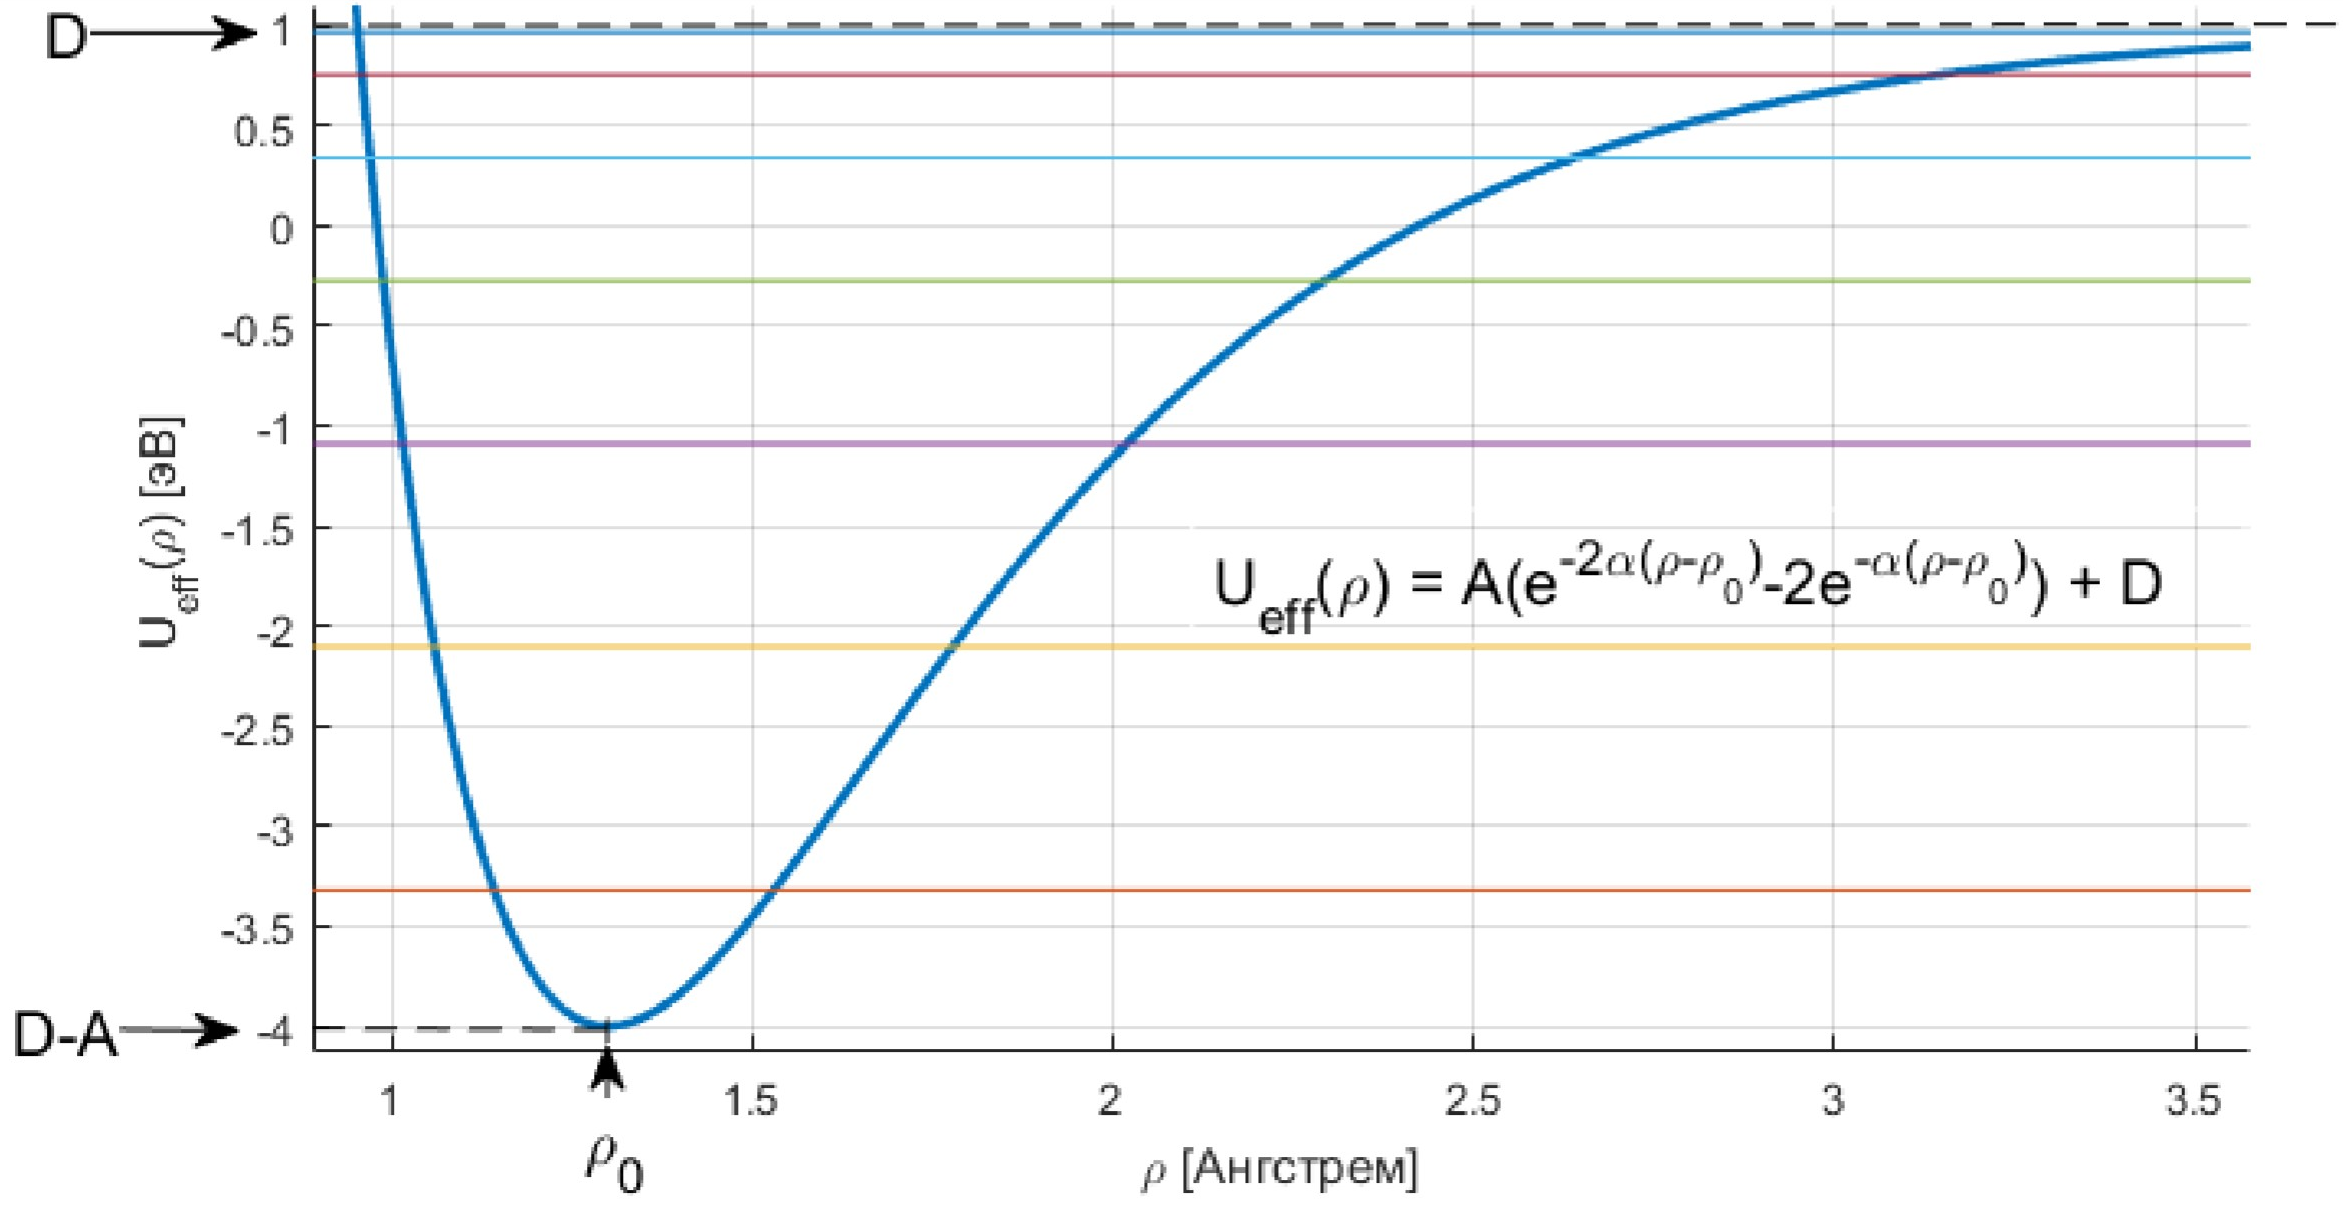
\includegraphics[width=\linewidth]{Morse.png}
	\caption{Вид кривой потенциала Морзе}
	\label{MorseGraph}
\end{figure}

На графике также показаны энергетические уровни стационарных
состояний для одномерного движения в таком потенциале, соответствующие колебательным термам. Отличительной особенностью энергетического спектра этого потенциала является конечное число дискретных уровней и уменьшение расстояния между соседними энергетическими уровнями с повышением номера уровня. Выражение для энергетического спектра движения в потенциале Морзе имеет вид:
\begin{equation}
E_n=D-A+\hbar\cdot{\alpha}\sqrt{\frac{2A}{\mu}}(n+\frac{1}{2})-\frac{\hbar^2\alpha^2}{2\mu}(n+\frac{1}{2})^2
\end{equation}
Обозначив частоту колебательного кванта $\omega_{\text{кол}}=\alpha\sqrt{\frac{2A}{\mu}}$ можно переписать в виде:
\begin{equation}
	E_n=D-A+\hbar \omega_{\text{кол}}(n+\frac{1}{2})-\frac{1}{4A}(\hbar \omega_{\text{кол}}(n+\frac{1}{2}))^2
\end{equation}
	Для анализа такого спектра полезно записать выражения для разностей между соседними уровнями $\Delta E_n=E_{n+1}-E_n$:
\begin{equation}
	E_n=\hbar \omega_{\text{кол}}-\frac{\hbar^2\alpha^2}{\mu}(n+1)=\hbar \omega_{\text{кол}}(1-\frac{\hbar\omega_{\text{кол}}}{2A}(n+1))
\end{equation}
\begin{equation}
	\Delta^2E_n=-\frac{\hbar^2\alpha^2}{\mu}
\end{equation}
	Для случая потенциала Морзе, значение вторых разностей одинаково для всего спектра, не зависит от номера $n$.  Используя выражения выше и экспериментально измеренный колебательный спектр можно вычислить микроскопические параметры $\alpha$ и $A$ описывающие взаимодействие между ядрами в двуатомной молекуле.
\subsection{Излучательные переходы между термами.}
Перестройка квантовой системы может сопровождаться электро-
магнитным излучением. Наибольшая вероятность излучения харак-
терна для переходов сопровождающихся изменением электрического
дипольного момента системы. Как известно из курса классической
электродинамики, мощность $P_{dp}$ электронного дипольного $\textbf{d}$ излучения определяется выражением:
\begin{equation}
	P_{dp}=\frac{2\ddot{\textbf{d}}^2}{3c^3}
\end{equation}
Рассмотрим квантовую систему у которой есть как минимум два
стационарных состояния $\ket{1}$ и $\ket{2}$, которые характеризуются волновыми функция и $\Psi_{1}(\vec{r},{t})$ и  $\Psi_{2}(\vec{r},{t})$ и соответствующими значениями энергии $E_1$ и $E_2$ . Изменение волновых функций во времени:
\begin{equation}
\begin{aligned}
	\Psi_{1}(\vec{r},{t})&=\psi_{1}(\vec{r})\cdot\exp\left(-i\frac{E_1}{\hbar}t\right)\\
	\Psi_{2}(\vec{r},{t})&=\psi_{2}(\vec{r})\cdot\exp\left(-i\frac{E_2}{\hbar}t\right)
\end{aligned}
\end{equation}
В течении перестройки квантовой системы, например, из состояния $\ket{1}$ в состояние $\ket{2}$ система находится в состоянии суперпозиции этих
двух состояний так, что волновая функция системы имеет вид:
\begin{equation}
	\Psi(\vec{r},{t})=\alpha\Psi_{1}(\vec{r},{t})+\beta\Psi_{2}(\vec{r},{t})
\end{equation}
при этом выполняется условие нормировки $|\alpha|^2+|\beta|^2=1$. Величина
электрического дипольного момента системы в промежуточном состоянии:
\begin{equation}
\textbf{d}={e}\cdot\textbf{r}={e}\cdot\int\Psi(\vec{{r}},{t})^{*}\hat{\textbf{r}}\Psi(\vec{{r}},{t})d^3\textbf{r}=|\alpha|^2\cdot\textbf{d}_{11}+|\beta|^2\cdot\textbf{d}_{22}+\alpha'\beta\textbf{d}_{12} +\alpha\beta'\textbf{d}_{21}
\end{equation}
Дипольные моменты $\textbf{d}_{1}$ и $\textbf{d}_{2}$ соответствуют стационарным состоя-
ниям и не изменяются во времени, а <<взаимные>> моменты $\textbf{d}_{12}$ и $\textbf{d}_{21}$ ыражаются комплексными числами, причём можно
установить, что эти значения комплексно-сопряжённые друг к другу: $\textbf{d}_{12} = \textbf{d}_{21}’$
\begin{equation}
\begin{aligned}
\textbf{d}_{12} = {e}\cdot exp(-{i}\frac{{E}_2-{E}_1}{\hbar}t)\int\psi_{1}(\vec{{r}})^{*}\textbf{r}\psi_{2}(\vec{{r}})d^3\textbf{r}=|\textbf{d}_{12}|\cdot{e}^{(-{i\omega}_{12}+i\varphi)}\\
\textbf{d}_{21} ={e}\cdot exp(-{i}\frac{{E}_1-{E}_2}{\hbar}t)\int\psi_{2}(\vec{{r}})^{*}\textbf{r}\psi_{1}(\vec{{r}})d^3\textbf{r}=|\textbf{d}_{21}|\cdot{e}^{(-{i\omega}_{21}+i\varphi)}
\end{aligned}
\end{equation}
где частота перехода $\omega_{12}=\frac{E_2-E_1}{\hbar}$, а угол $\varphi$ означает фазу интеграла $\int\psi_1(\vec{r})^*\hat{\textbf{r}}\psi_2(\vec{r})d^3\textbf{r}$.

Эволюция во времени волновой функции от состояния $\ket{1}$ в состояние $\ket{2}$ описывается зависимостью коэффициентов $\alpha$ и $\beta$ от времени с сохранением условия нормировки. Вид функций от времени для этих коэффициентовдолженопределятьсяисходяизвременногоуравнения Шрёдингера с подходящей моделью взаимодействия квантовой системы с электромагнитным полем. В случае электромагнитного поля низкой интенсивности время излучательного перехода как правило много больше чем период одного колебания. Тогда, приближённо считая коэффициенты $\alpha$ и $\beta$ постоянными во времени, получим следующее выражение для второй производной дипольного момента:
\begin{equation}
	\ddot{\textbf{d}}=\beta'\alpha\cdot\ddot{\textbf{d}}_{21}+\alpha'\beta\cdot\ddot{\textbf{d}}_{12}=2\text{Re}\left(\alpha'\beta\cdot\frac{d^2\textbf{d}_{12}}{dt^2}\right)=-2|\textbf{d}_{12}|\omega^2_{12}\text{Re}(\alpha'\beta)\cdot\cos(\omega_{12}t+\varphi)
\end{equation}
И для мощности дипольного излучения:
\begin{equation}
	P_{dp}=\frac{2\ddot{\textbf{d}}^2}{3c^3}=\frac{8|\textbf{d}_{12}|^2\text{Re}^2(\alpha'\beta)}{3c^2}\omega_{12}^4\cdot\cos^2(\omega_{12}t+\varphi)
\end{equation}
Из этого выражения видно, что мощность дипольного излучения зависит от произведения коэффициентов $\alpha$ и $\beta$, и от квадрата модуля матричного элемента оператора дипольного момента $|\textbf{d}_{12}|^2$.
\subsection{Принцип Франка-Кондона}
Как отмечено выше, различные состояния электронной подсистемы соответствуют различным электронным термам молекулы. Переходы между электронными термами могут сопровождаться электромагнитным излучением на частотах вблизи видимого диапазона. Точное значение частоты излучения определяется не только электронными термами начального и конечного состояний молекулы, но также соответствующими колебательными и вращательными термами.
\begin{figure}[h]
\centering
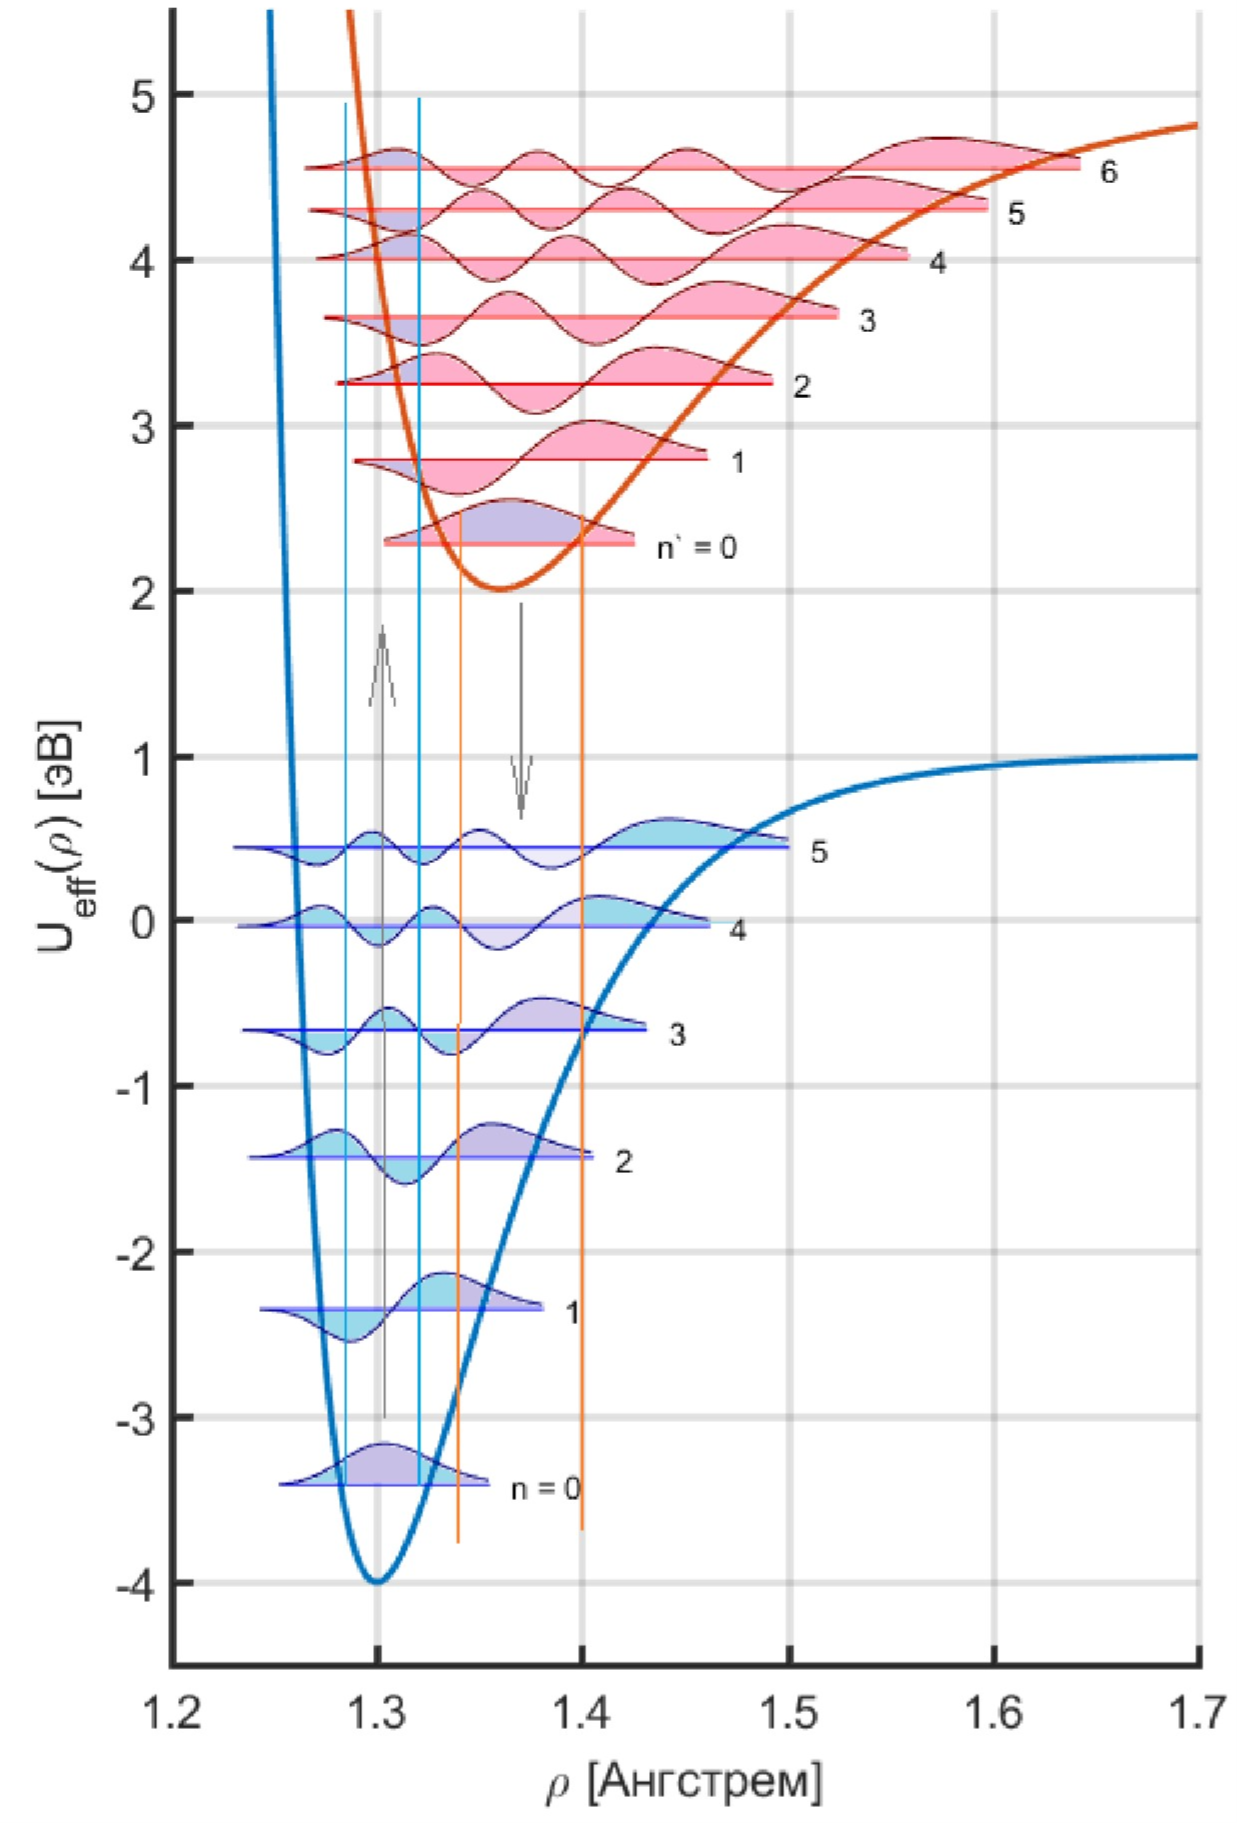
\includegraphics[scale=0.5]{Therms.png}
\caption{Электронно-колебательные термы и переходы}
\label{fig:Therms}
\end{figure}

Вероятность излучательного перехода зависит от матричного элемента $|\textbf{d}_{12}|^2$. Для сферически симметричных систем условие $|\textbf{d}_{12}|^2\neq 0$ приводит к так называемым правилам отбора, которые связаны с законом сохранения момента импульса и чётности квантового состояния. Но для двухатомных молекул возникает специфическое  правило, определяющее вероятность излучательного перехода, -- так называемый принцип Франка-Кондона.

Для пояснения этого принципа запишем выражение для матричного элемента $|\textbf{d}_{12}|^2$ дипольного момента двухатомной молекулы:
\begin{equation}
	\textbf{d}_{21}=\int\Psi_2(\{\vec{R}\},\{\vec{r}\})^*\hat{r}\Psi_1(\{\vec{R}\},\{\vec{r}\})d^{3n}\{\textbf{r}\}d^6\{\textbf{R}\}
\end{equation}
где $n$ - количество электронов в двухатомной молекуле. Используя, в соответствии с (\ref{eq:1}) запись волновой функции молекулы в виде произведения волновых функций ядерной и электронной подсистем, получим:
\begin{equation}
\begin{aligned}
\int\Phi_2(\vec{R}_1,\vec{R}_2)^*\Phi_1(\vec{R}_1,\vec{R}_2)d^3\textbf{R}_1d^3\textbf{R}_2\cdot\int\psi_2(\{\vec{r}\})^*\hat{\textbf{r}}\psi_1(\{\vec{r}\})d^{3n}\{\textbf{r}\}=\\
=\int\Psi_2^{nuc}(\vec{\rho})^*\Psi_2^{nuc}(\vec{\rho})d^3\vec{\rho}\cdot\textbf{d}_{21}^{el}=\\
=\int\psi_2^{nuc}(\rho)^*\psi_1^{nuc}(\rho)d^{\rho}\int Y^{nuc}_{l_2,m_2}(\theta,\varphi)^*Y^{nuc}_{l_1,m_1}(\theta,\varphi)\sin(\theta)d\theta d\varphi\cdot\textbf{d}_{21}^{el}=\\
=\int\psi^{nuc}_2(\rho)^*\psi_1^{nuc}(\rho)d^{\rho}\cdot\delta_{m_1,m_2}\delta_{l_1,l_2}\cdot\textbf{d}_{21}^{el}
\end{aligned}
\end{equation}
Для пояснения этого принципа на рисунке \ref{fig:Therms} показаны \textbf{потенциальные кривые} двух различных электронных термов, а также колебательные термы каждого электронного состояния. Вращательные термы не показаны. Помимо энергетических уровней стрелочками обозначена серия поглощающих переходов $(n-n')$ и серия испускающих переходов $(n'-n)$.

В наиболее простой формулировке принцип Франка-Кондона гласит, что интеграл перекрытия волновых функций состояний $(n)$ и $(n')$ определяетвероятностьизлучательногопереходамеждуэтимисостояниями, и чем выше значения этого интеграла $\bra{n}\ket{n'}$, тем выше вероятность излучательного перехода. Для колебательных термов с большим значением номера уровня n приближённо можно считать, что волновая функция имеет неосциллирующий характер только вблизи точек поворота соответствующих квазиклассических траекторий. Поэтому интегралыперекрытиядлятакихтермовбудутсущественноотличаться от нуля, если для этих состояний точки разворота близки друг к другу.
\newpage
\section{Экспериментальная установка}
\subsection{Устройство трехпризменного стеклянного спектрографа ИСП-51}
\begin{figure}[!htb]
\centering
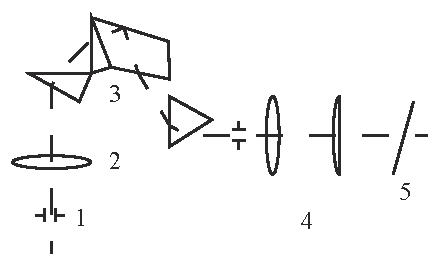
\includegraphics[scale=1]{scheme.pdf}
\caption{Устройство спектрографа}
\label{fig:scheme}
\end{figure}
Оптическая схема прибора показана на рисунке \ref{fig:scheme}, где 1 - входная щель коллиматора с шириной раскрытия до 0,4 мм и отсчетом по барабанчику с ценой деления 0,001мм; 2 - коллиматор; 3 - диспергирующая система прибора; 4 - объектив фотокамеры; 5 - поверхность изображения спектра.

Свет от источника, пройдя через входную щель и коллиматор прибора, параллельным пучком падает на диспергирующую систему призм, которая разлагает пучок белого света в спектр и одновременно поворачивает осевой луч под прямым углом. Разложенный пучок света с помощбю объектива фотокамеры фокусируется в плоскость матрицы.

\subsection{Схема экспериментальной установки}
        На рисунке приведена блок-схема установки. Вработе используются поочередно два источника излучения: лампа накаливания 1 - для изучения спектров пропускания и ртутная лампа 6 - для калибровки регистрирующей аппаратуры. Пары йода образуются в результате сублимации кристаллов йода, находящихся в кювете 4 и подогреваемых нихромной спиралью, подключенной вместе с лампой накаливания к блоку питания. Излучение лампы накаливания фокусируется линзой 3 на входную щель 7 спектрографа ИСП-51 которая разлагает его в спектр. В фокально плоскости спектрографа устанавливается фотоаппарат Nikon D5300
\begin{figure}[!htb]
	\centering
	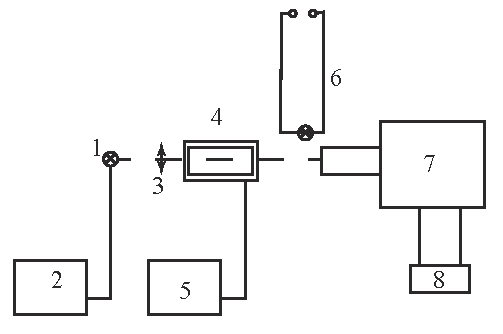
\includegraphics[scale=1]{experiment.pdf}
	\caption{Схема установки}
\end{figure}

        2 и 5 -- это блоки питания. В нашей работе спектр поглощения паров йода наблюдается визуально на фоне сплошного спектра лампы накаливания , питаемой от блока питания 
	    
	    Кювета с кристаллами йода подогревается нихромовой спиралью, подключённой вместе с лампой накаливания к блоку питания. Линза используется как конденсор.
	    
	    В результате подогрева кристаллы йода частично возгоняются, образуя пары с лёгкой фиолетовой окраской. Спектрометр позволяет визуально наблюдать линии поглощения молекул йода на фоне сплошного спектра излучения лампы накаливания видимой области.
\section{Ход работы}
\subsection{Калибровка спектрографа}
Для начала снимем спектр ртутной лампы, используемой для калибровки спектрографа. Полученный спектр изображен на рис. \ref{hg_spec}.
\begin{figure}[!htb]
	\centering
	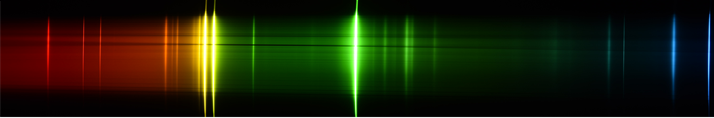
\includegraphics[width=\textwidth]{hg_lamp.png}
	\caption{Снимок калибровочного спектра}
	\label{hg_spec}
\end{figure}\\
С помощью атласа линий ртути сопоставим линии излучения с номером пикселя и построим график зависимости длины волны от номера пикселя. Полученная зависимост изображена на рис. \ref{plot1}.
\begin{figure}[!htb]
	\centering
	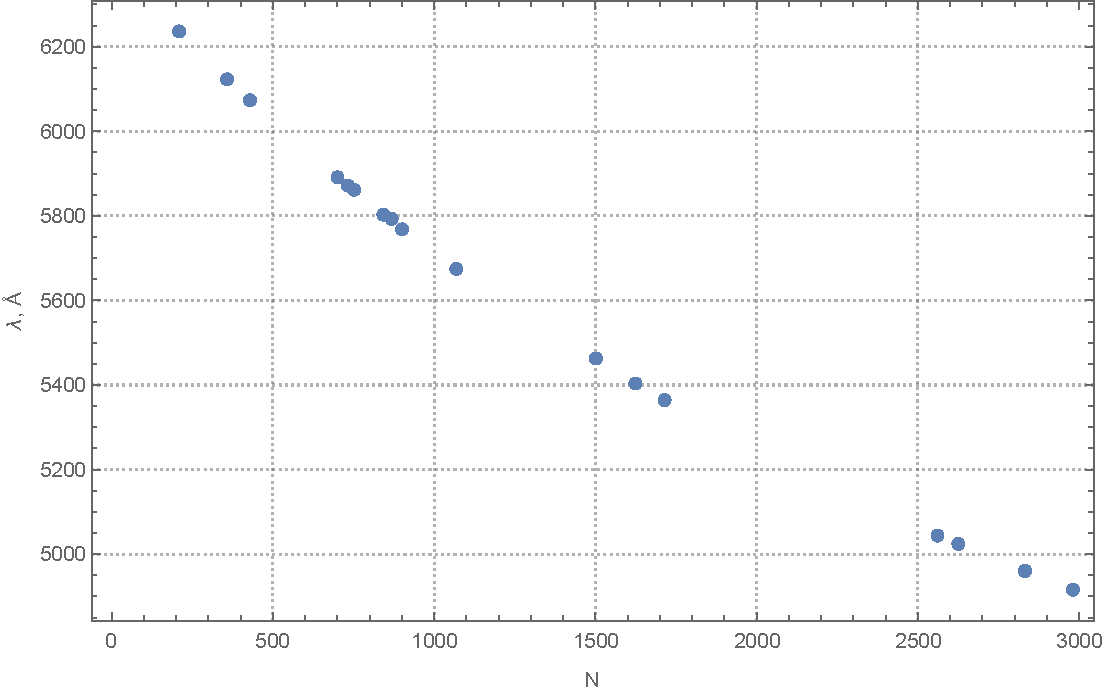
\includegraphics[scale=0.7]{plot1.pdf}
	\caption{Зависиомсть длинны волны от номера пикселя}
	\label{plot1}
\end{figure}\\
Аппроксимируем точки. Формула для калибровки имеет вид $f(x)=a+\frac{c}{x-b}$. Методом наименьших квадратов найдем значения параметров $a,\ b$ и $c$. Таким образом получили значения: $a=2889.97$, $b= -4060.89$, $c=1.43\cdot10^7$. Сведем на один график полученную кривую и экспериментальную зависимость длин волн излчения от номера пикселя (рис. \ref{plot2}).
\begin{figure}[h]
	\centering
	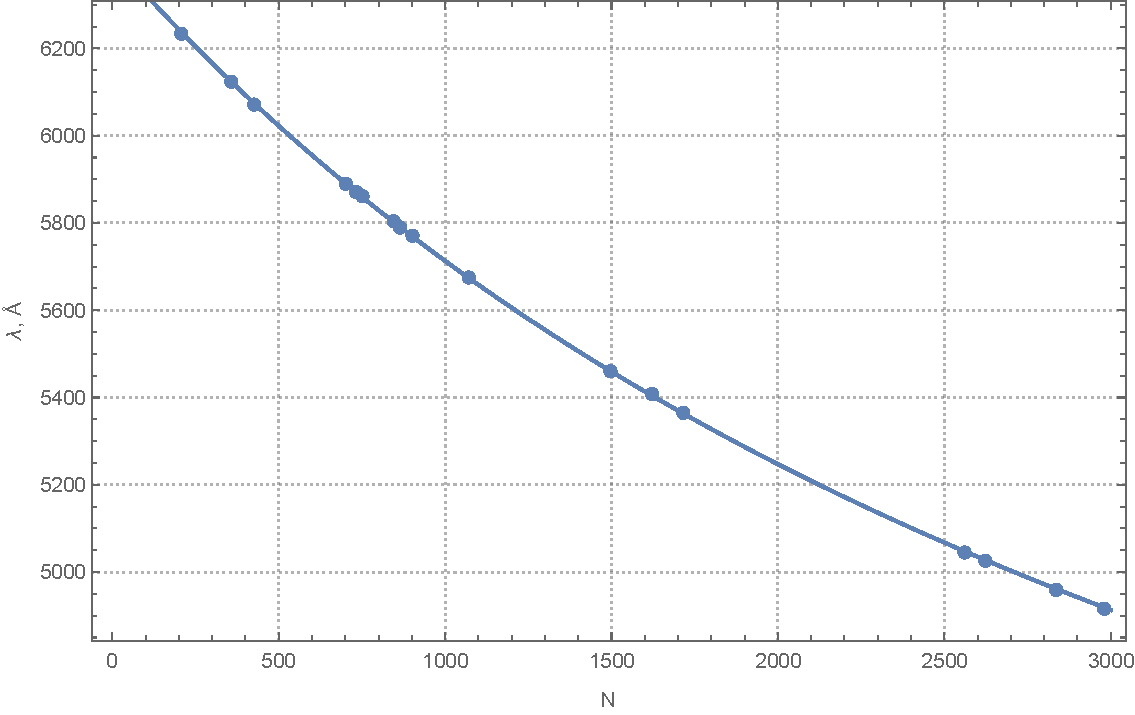
\includegraphics[scale=0.7]{plot2.pdf}
	\caption{Полученная калибровочная кривая}
	\label{plot2}
\end{figure}
\subsection{Получение и обработка спектра поглощения I$_2$}
Установив лампу накаливания и кювету с йодом, зафиксируем изображение спектра поглощения I$_2$. Полученный спектр изображен на рис. \ref{i2_spec}.
\begin{figure}[!htb]
	\centering
	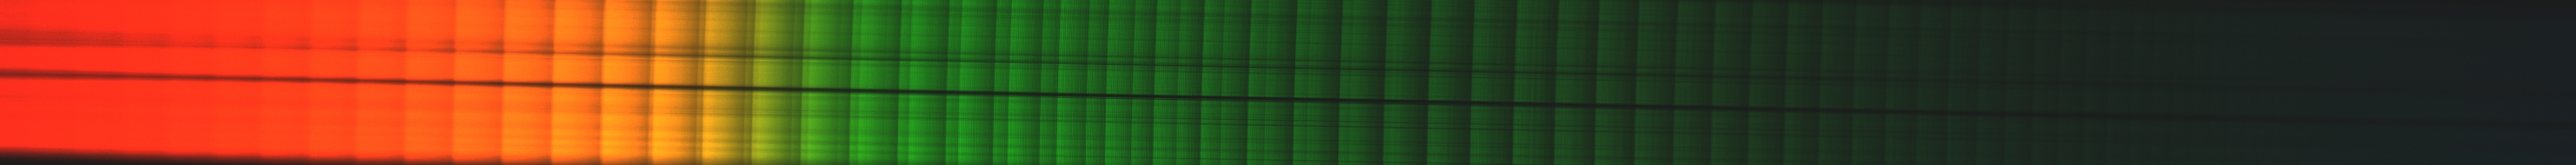
\includegraphics[width=\textwidth]{i2.jpeg}
	\caption{Полученный спектр поглощения I$_2$}
	\label{i2_spec}
\end{figure}

\end{document}